\section{Introduction}
\subsection{Deliberation for logistic}

\begin{frame}{Scientific study domains}
    \centering
\begin{columns}
    \begin{column}{0.5\textwidth}
        Study field of the authors 
        \small
        \begin{itemize}
            \item Hierarchical and temporal planning techniques.
            \item Robotic architecture.
            \item Cooperation in complex and large environment.
        \end{itemize}
        Focus on deliberation in logistic problems: 
        \small
        \begin{itemize}
            \item Scheduling,
            \item Robot control,
            \item Fleet Management,
            \item Resource allocation.
        \end{itemize}
    \end{column}
    \begin{column}{0.5\textwidth}
        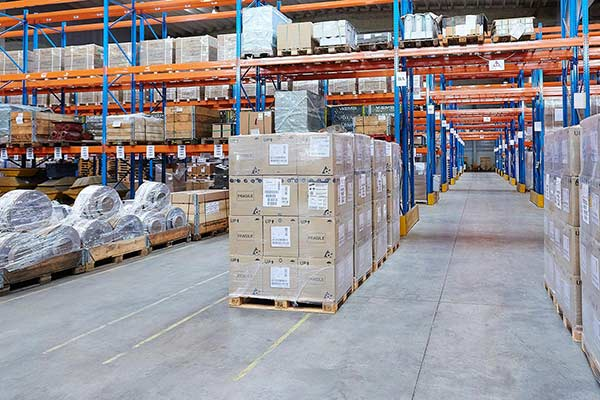
\includegraphics[width = \textwidth]{images/logisticsolutions.jpg}
    \end{column}
\end{columns}

\end{frame}

\begin{frame}{Factory simulator for logistic problems}
    GobotSim, a new simulator for logistic problems.

    ~


    \begin{columns}
        \begin{column}{0.5\textwidth}
            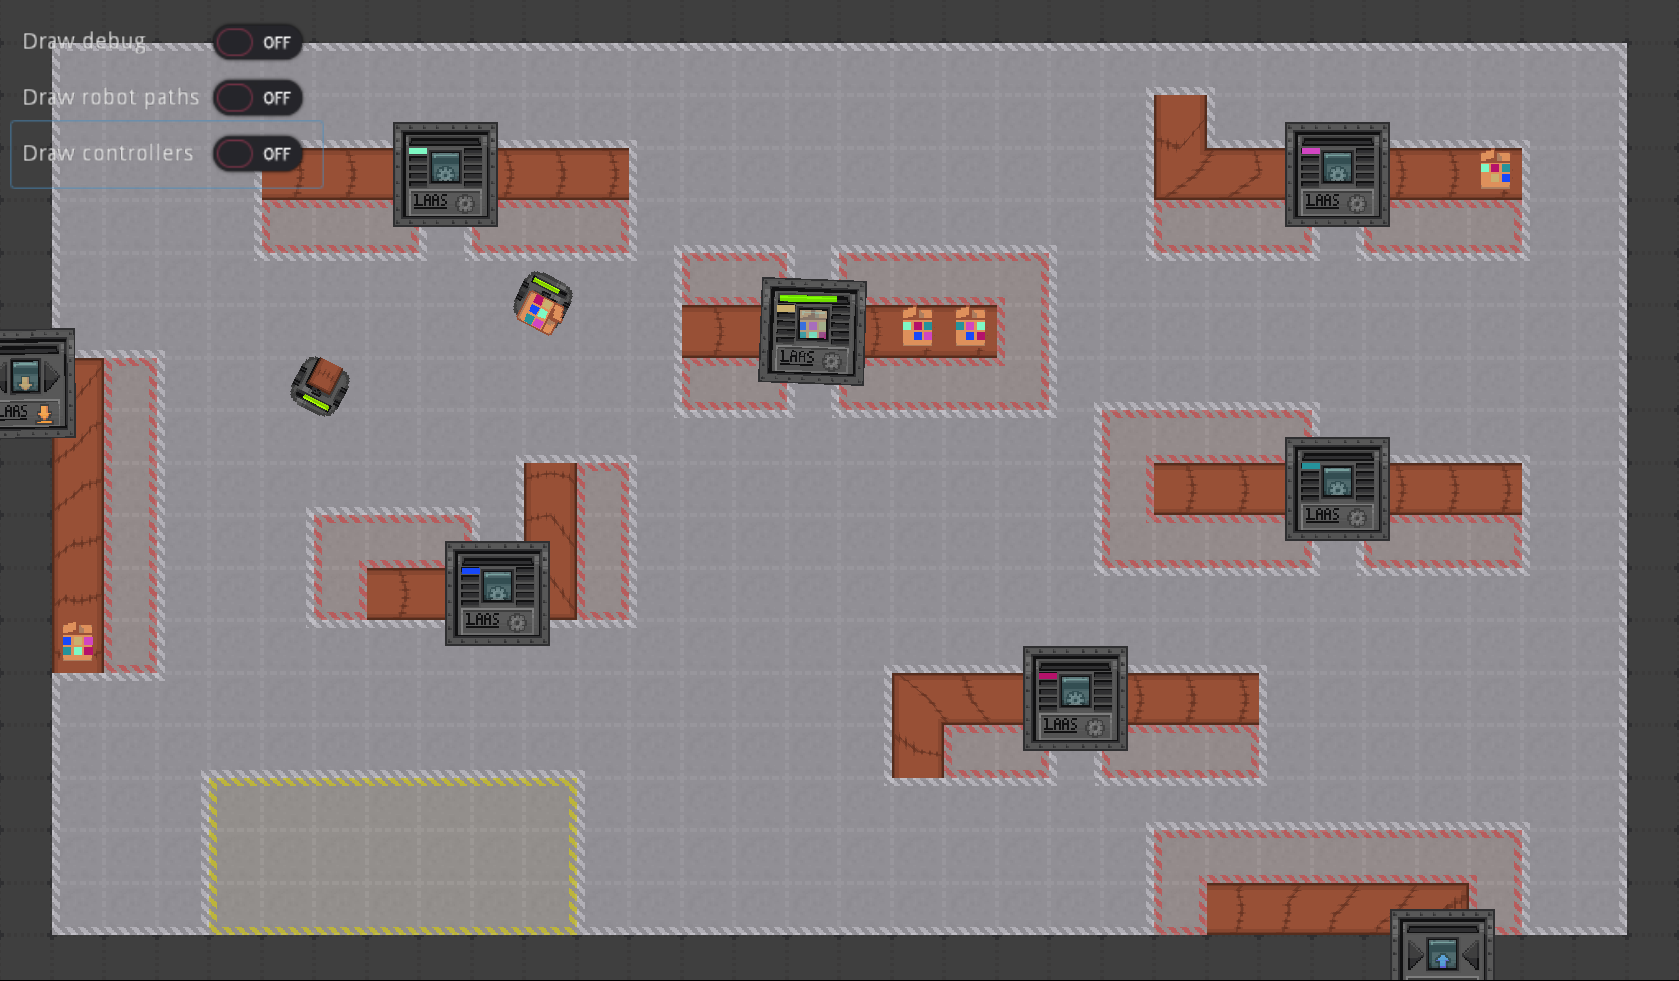
\includegraphics[width=\linewidth]{images/gobot-rae.png}
        \end{column}
        \begin{column}{0.5\textwidth}
            Emphasis on
            \begin{itemize}
                \item Deliberation aspects
                \item Logistic problematics: scheduling, resource
            \end{itemize}
            
            Compaired to existing simulators:
            \begin{itemize}
                \item RoboCup: Manipulation, cooperation
                \item Craft-bots: Exploration, resource gathering
            \end{itemize}
        \end{column}
    \end{columns}
\end{frame}

\begin{frame}{GobotSim environment}
    \begin{columns}
        \begin{column}{0.2\textwidth}
            
\includegraphics[width = 0.8\textwidth]{images/godot/machine_texture.png}
        \end{column}
        \begin{column}{0.7\textwidth}
            Machines
            \begin{itemize}
                \item Processing : does a predefined list of process for packages
                \item Input: generate packages
                \item Output: gather fully processed packages
            \end{itemize}

        \end{column}
    \end{columns}

    \begin{columns}
        \begin{column}{0.2\textwidth}
            
\includegraphics[width = 0.8\textwidth]{images/godot/robot_texture.png}
        \end{column}
        \begin{column}{0.7\textwidth}
            Robots : manipulate packages
            \begin{itemize}
                \item commands: move, pick, place,\dots
                \item recharge at recharge areas
            \end{itemize}
        \end{column}
    \end{columns}
\end{frame}

\subsection{Single agent scenario}


\begin{frame}{Simple scenario: one package}
    \centering
    \begin{columns}
        \begin{column}{0.5\textwidth}
            \centering
            
\includegraphics[width = 0.5\textwidth]{images/godot/package.png}
            
            \LARGE \emph{$\times 1$}
        \end{column}
        \begin{column}{0.5\textwidth}
            \centering
            
\includegraphics[width = 0.5\textwidth]{images/godot/robot_texture.png}
            
            \LARGE \emph{$\times 1$}
        \end{column}
    \end{columns}
\end{frame}

\begin{frame}{Definition of a robotic agent}

    \begin{columns}[T]
        \begin{column}{0.3\textwidth}
            An entity

            ~

            
\includegraphics[width = 0.7\textwidth]{images/icons8-robot-gustav-500.png}
        \end{column}
        \begin{column}{0.7\textwidth}
            \center Capable of :
            \pause
            \begin{enumerate}
                \item Perceiving its environment
                \pause
                \item Modifying its environment (actions)
                \pause
                \item \textbf{Deliberating:} Reasoning about its \textbf{skills} in order to fulfill a goal
            \end{enumerate}
        \end{column}
    \end{columns}

 
\end{frame}

\begin{frame}{Hierarchical operational models to represent the capabilities of an agent}

\begin{columns}[T]
    \begin{column}{0.55\textwidth}

        \begin{itemize}
            \item Elementary capabilities : move, pick, place, \dots
            \pause
            \item Skills : executable programs (operational models): transport, process \dots
            \pause
            \item Agent behavior = composition of skills
        \end{itemize}
        
        ~
        \pause
        Acting domain \textbf{$A_\Delta (A, T, M_t)$}: Hierarchical operational models
        \small
        \pause
        \begin{itemize}
        
        
         \item[$A$] : commands
         \pause
         \item[$T$] : tasks
         \pause
         \item[$M_t$] : methods: pre-conditions, body (operational model)
         
     \end{itemize}
    \end{column}
    \pause
    \begin{column}{0.45\textwidth}
        \begin{figure}
            \begin{tikzpicture}
                \node[draw,ellipse, ultra thick] (t) {\textit{open door}} [sibling distance = 3.5cm]
                  child {node[draw, ultra thick] (m1) {$m_1$} edge from parent [dashed]
                  child {node[draw,rounded corners, ultra thick, solid] (a1) {$push$} edge from parent
                  }} 
                  child {node[draw, ultra thick] (m2) {$m_2$} edge from parent [dashed] [sibling distance = 1.5cm]
                  child {node[draw, rounded corners, solid, ultra thick] (a2) {grab handle} edge from parent [solid]}
                  child {node[draw, rounded corners, solid, ultra thick] {$pull$} edge from parent [solid]}};
                \node[right = 0em of t] {$\in T$};
                \node[right = 0em of m1] {$\in M_t$};
                \node[right = 0em of m2] {$\in M_t$};
                \node[right = 0em of a1] {$\in A$};

            \end{tikzpicture}
            \caption{Example of hierarchy for the \textit{task} \textit{open door}}

            
        \end{figure}
    \end{column}
\end{columns}
    
\end{frame}

\begin{frame}{Deliberate using hierarchical operatinal models with the Refinement Acting Engine (RAE)\footnote{Automated Planning and Acting \cite{ghallabAutomatedPlanningActing2016}}}
    RAE features:
    \begin{itemize}
        \item Monitor command and task execution in parallel.
        \item Refine tasks at runtime to select a suitable method with its parameters depending on the context
        
        \begin{tikzpicture}
            \node[] (task) {$\tau(p_1,\dots,p_n)$};
            \node[below = 2em of task] (method) {$m(p_1,\dots,p_n, \dots, p_m)$};
            \path[->] (task) edge node[right, midway] {refinement} (method);
        \end{tikzpicture}
    \end{itemize}    
\end{frame}
    

\begin{frame}{Refinement Acting Engine algorithms}
    \begin{columns}[T]
  
        \begin{column}{0.65\textwidth}
            
            Algorithms:
            \small
            \begin{itemize}
                \setlength{\leftmargini}{-1pt}
                \onslide<2->
                \item \textbf{Main:} 
                \begin{itemize}
                    \item Receive $\tau$ (task or event);
                    
                    add it to the \textbf{agenda} (ongoing tasks)
                    \onslide<3->
                    \item Refine $\tau$: \textbf{Select} an applicable method $m$ for $\tau$
                    \onslide<4->
                    \item \textbf{Progress} $m$
                \end{itemize}
                \onslide<5->
                \item \textbf{Progress:}
                    \begin{itemize}
                        \onslide<6->
                        \item Monitor execution of $m$.
                        \onslide<7->
                        \item Refine subtasks in $m$.    
                        \onslide<8->
                        \item Monitor execution of subtasks.
                        \onslide<9->
                        \item \textbf{Retry} $\tau$ in case of \emph{failure}:
                    
                    Call \textbf{Select} to get a new method;
                    
                    \textbf{Progress} the new method.
                    \end{itemize}
            \end{itemize}
        \end{column}
        \begin{column}{0.35\textwidth}
            \begin{tikzpicture}
                \onslide<2>
                \node[draw,ellipse, ultra thick] (t) {$\tau$};
                \onslide<3-9>
                \node[draw,ellipse, ultra thick, color = orange] (t) {$\tau$};
                \onslide<10>
                \node[draw,ellipse, ultra thick, color = green] (t) {$\tau$};
                \onslide<3>
                \node[draw, ultra thick, below= 2em of t, xshift = -3em] (m1) {$m_1$};
                \node[draw, ultra thick, below= 2em of t, xshift = 3em] (m2) {$m_2$};
                \onslide<4->
                \node[draw, ultra thick, below= 2em of t, xshift = -3em, color = orange] (m1) {$m_1$};
                \node[draw, ultra thick, below= 2em of t, xshift = 3em, color = gray] (m2) {$m_2$};
                \onslide<10>
                \node[draw, ultra thick, below= 2em of t, xshift = -3em, color = green] (m1) {$m_1$};
                \onslide<3->
                \path[-] (t) edge (m1) (t) edge (m2);
                \onslide<5>
                \node[draw,rounded corners, ultra thick, solid, below = 2em of m1, xshift = -1.5em] (a1) {$a1$};
                \onslide<6>
                \node[draw,rounded corners, ultra thick, solid, below = 2em of m1, xshift = -1.5em, color = orange] (a1) {$a1$};
                \onslide<7->
                \node[draw,rounded corners, ultra thick, solid, below = 2em of m1, xshift = -1.5em, color = green] (a1) {$a1$};
                \onslide<5-7>
                \node[draw,ellipse, ultra thick, solid, below = 2em of m1, xshift = 1.5em] (t2) {$\tau_s$};
                \onslide<8->
                \node[draw,ellipse, ultra thick, solid, below = 2em of m1, xshift = 1.5em, color = orange] (t2) {$\tau_s$};
                \onslide<10>
                \node[draw,ellipse, ultra thick, solid, below = 2em of m1, xshift = 1.5em, color = green] (t2) {$\tau_s$};
  
  
                \onslide<5->
                \path[-] (m1) edge (a1) (m1) edge(t2);
  
  
                \onslide<7>
                \node[draw, ultra thick, below = 2em of t2, xshift = -1.5em] (m3) {$m_3$};
                \node[draw, ultra thick, below = 2em of t2, xshift = 1.5em] (m4) {$m_4$};
                \path[-] (t2) edge  (m3) (t2) edge (m4);
                
                \onslide<8>
                \node[draw, ultra thick, below = 2em of t2, xshift = -1.5em, color = orange] (m3) {$m_3$};
                \node[draw, ultra thick, below = 2em of t2, xshift = 1.5em, color = gray] (m4) {$m_4$};
                \path[-] (t2) edge  (m3) (t2) edge (m4);
  
                \onslide<9->
                \node[draw, ultra thick, below = 2em of t2, xshift = -1.5em, color = red] (m3) {$m_3$};
                \node[draw, ultra thick, below = 2em of t2, xshift = 1.5em, color = orange] (m4) {$m_4$};
                \path[-] (t2) edge  (m3) (t2) edge (m4);
                \onslide<10>
                \node[draw, ultra thick, below = 2em of t2, xshift = 1.5em, color = green] (m4) {$m_4$};
                
                \onslide<8->
                \node[below = 2em of m3, xshift = -1em] (e3) {};
                \node[below = 2em of m3, xshift = 1em] (e4) {};
                \path[-] (m3) edge  (e3) (m3) edge (e4);
  
                \onslide<8->
                \node[below = 2em of m4, xshift = -1em] (e5) {};
                \node[below = 2em of m4, xshift = 1em] (e6) {};
                \path[-] (m4) edge  (e5) (m4) edge (e6);
      
            \end{tikzpicture}
        \end{column}
    \end{columns}    
\end{frame}

\begin{frame}{RAE models for one package and one robot}
    \begin{itemize}
        \item Run example.
        \item High-level models.
    \end{itemize}
\end{frame}

\subsection{Multi-agent scenario}

\begin{frame}{Several packages?}
    \begin{columns}
        \begin{column}{0.5\textwidth}
            \centering
            
\includegraphics[width = 0.5\textwidth]{images/godot/package.png}
            
            \Large $\times n$
        \end{column}
        \begin{column}{0.5\textwidth}
            \centering
            
\includegraphics[width = 0.5\textwidth]{images/godot/robot_texture.png}
            
            \LARGE $\times m$
        \end{column}
    \end{columns}
    
    In function of n and m, deliberation must:
    \begin{itemize}
        \item Schedule package passage on machines
        \item Allocate package displacement tasks to robots
        \item Monitor the robots' batteries 
    \end{itemize}
\end{frame}

\begin{frame}{How to deliberate with multiple agents in parallel?}
    \begin{columns}
        \begin{column}{0.45\textwidth}
            RAE shortcomings:
            \begin{itemize}
                \item Progression of tasks relies on Round Robin
                \item Methods limited to a sequence of actions
                \item Difficulties to integrate sound planning from operational models due to implementation in Python.
            \end{itemize}
        \end{column}
        $\rightarrow$
        \pause
        \begin{column}{0.45\textwidth}
            Adapt RAE for multi-agents to
            \begin{itemize}
                \item Deal with concurrency
                \item Improve the interleaving of parallel tasks
                \item Reason on shared resources to optimize the overall process
            \end{itemize}
        \end{column}
    \end{columns}
\end{frame}